%!TEX root = ../thesis.tex

\chapter{Umsetzung}
\label{chap:umsetzung}

Im nachfolgenden wird die Konzeption und Umsetzung der in \ref{sec:anforderungsanalyse}
beschriebenen Anforderungen an das Projekt \projectname{} erläutert.
Der Schwerpunkt soll dabei speziell auf die Cross Plattform Architektur sowie auf die
Entwicklung der Komponenten hinsichtlich wiederverwendbarkeit gerichtet werden.


\section{Konzeption der Applikationsstruktur}

In diesem Kapitel wird die Konzeptphase der Plattformübergreifenden Applikationsstruktur (Abbildung \ref{kapitel4/arch}) erläutert.
Um Endprodukte für Web, Desktop und App zu generieren werden die Frameworks Angular 2, Electron und das
Ionic \ac{SDK} verwendet. Die Codebase für die Web- und Desktop Anwendung lassen sich so weit vereinen,
dass diese sich ein gemeinsames Repository teilen. Ein weiteres Repository beinhaltet die hybride Applikation,
welche mithilfe des Ionic 2 \ac{SDK} entwickelt wird. Obwohl Ionic 2 auf das Angular Framework aufbaut,
macht es Sinn den Web und App Code voneinander getrennt zu behandeln.
Gründe dafür sind zum einen konzeptionelle Unterschiede zwischen Web und App von \projectname{}.
Darüber hinaus unterscheiden sich die Navigation APIs der Frameworks, sowie die Menüführung der beiden Anwendungen.
Die \ac{UI} und Funktionalität wird daher innerhalb der Angular 2 (Web/Desktop)
Anwendung in Form von wiederverwendbaren Komponenten entwickelt und
Repository-übergreifend für die Verwendung im Ionic 2 Projekt verteilt.
Der verteilte Code wird im folgenden als \textbf{Shared Layer} bezeichnet.
Das Shared Layer beinhaltet verschiedene Elemente, welche die Kernfunktionalitäten von \projectname{} abdecken.
Im Folgenden werden zwischen View-Komponenten und wiederverwendbaren Komponenten sowie Service Implementierungen unterschieden.


\begin{itemize}
  \item Angular 2/Web und Desktop: github.com/michaelknoch/mia
  \item Ionic 2/App: github.com/michaelknoch/miamobile
\end{itemize}



\begin{figure}[h]
 \centering
 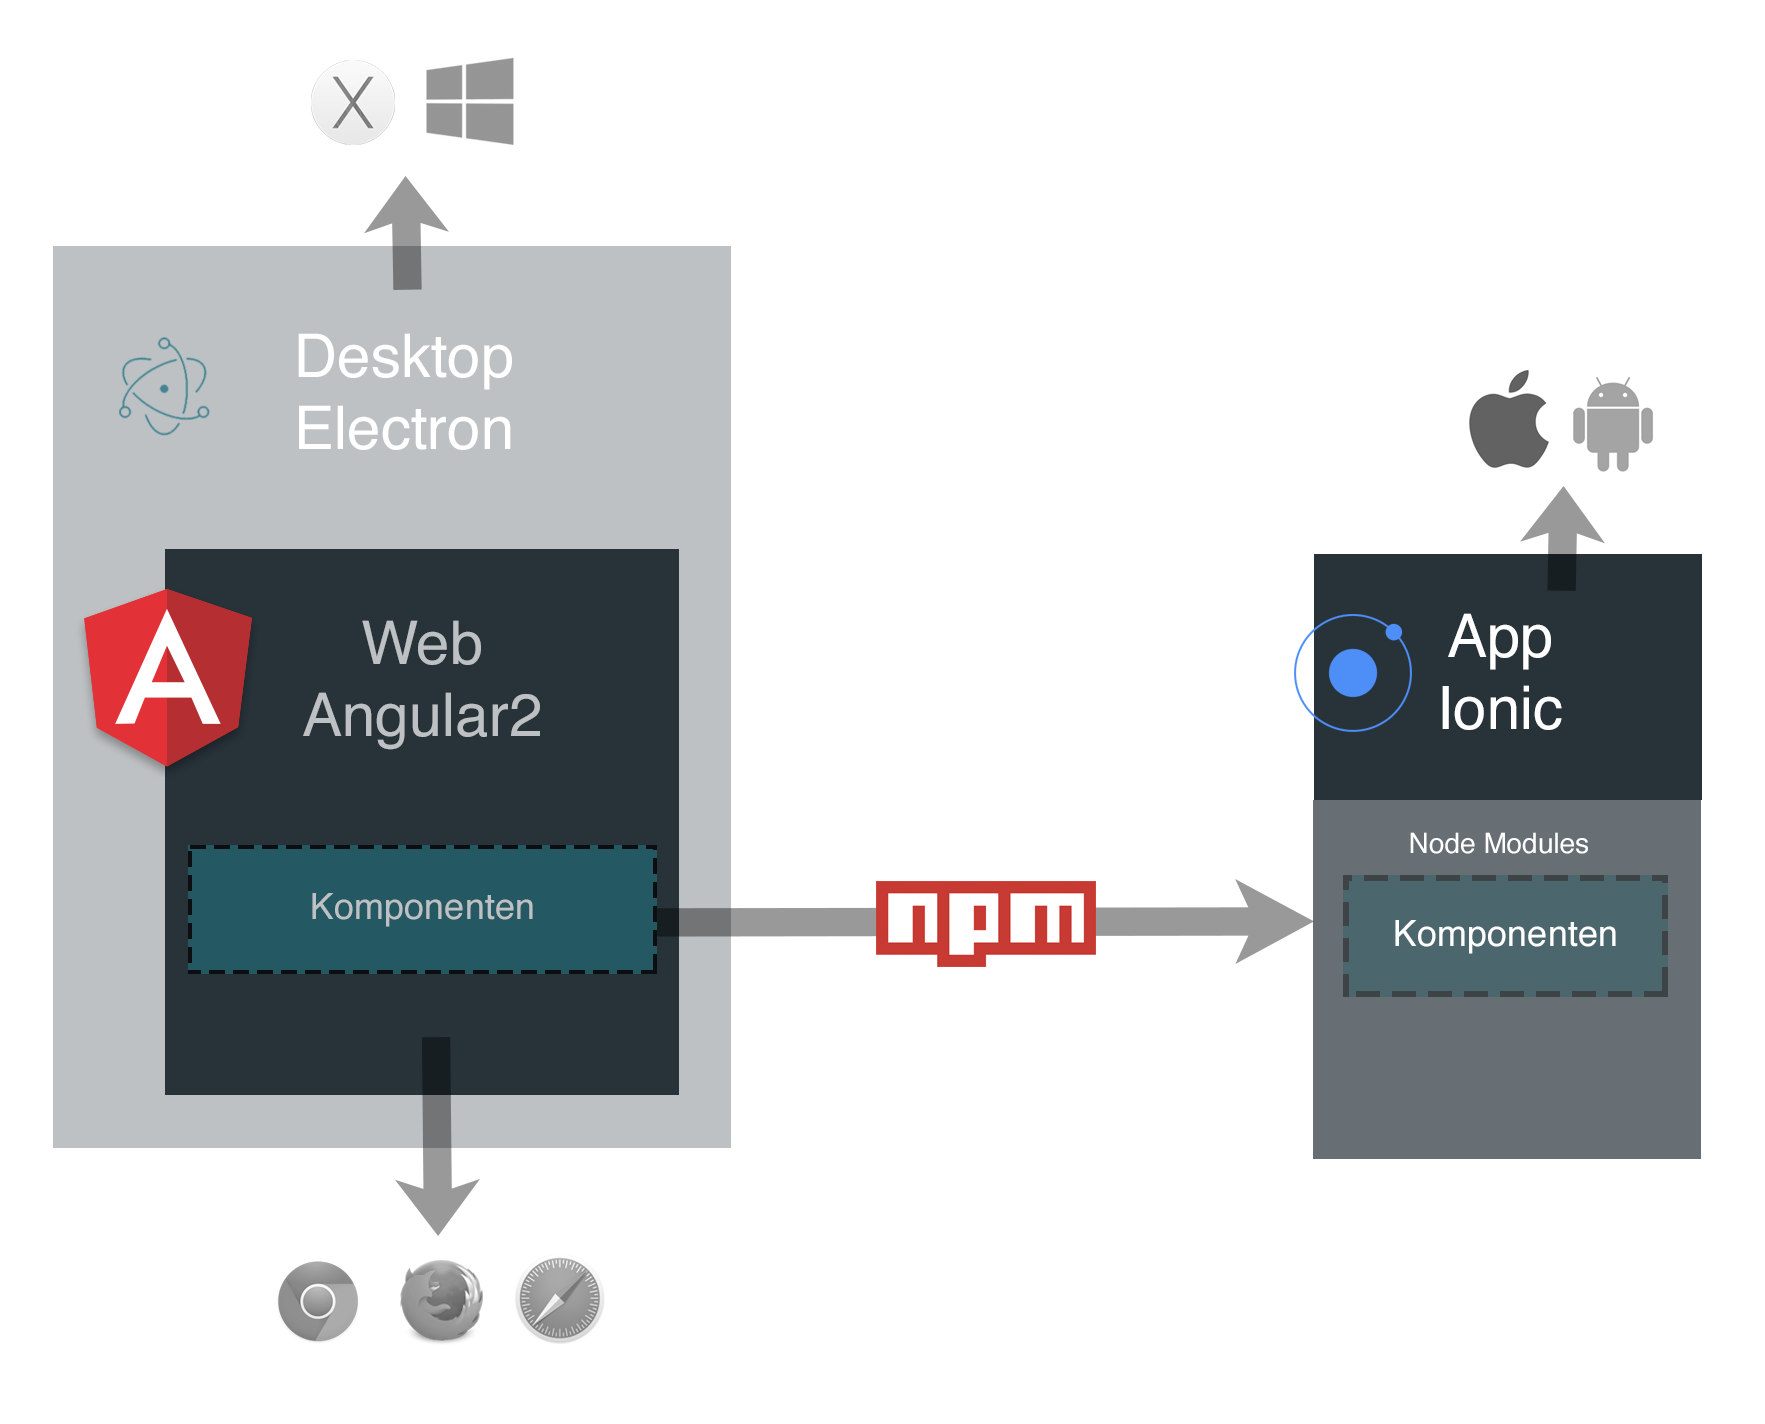
\includegraphics[width=\linewidth]{kapitel4/arch.png}
 \caption{Cross Plattform Architektur}
 \label{kapitel4/arch}
\end{figure}
\vspace{0.3cm}




\begin{figure}[h]
 \centering
 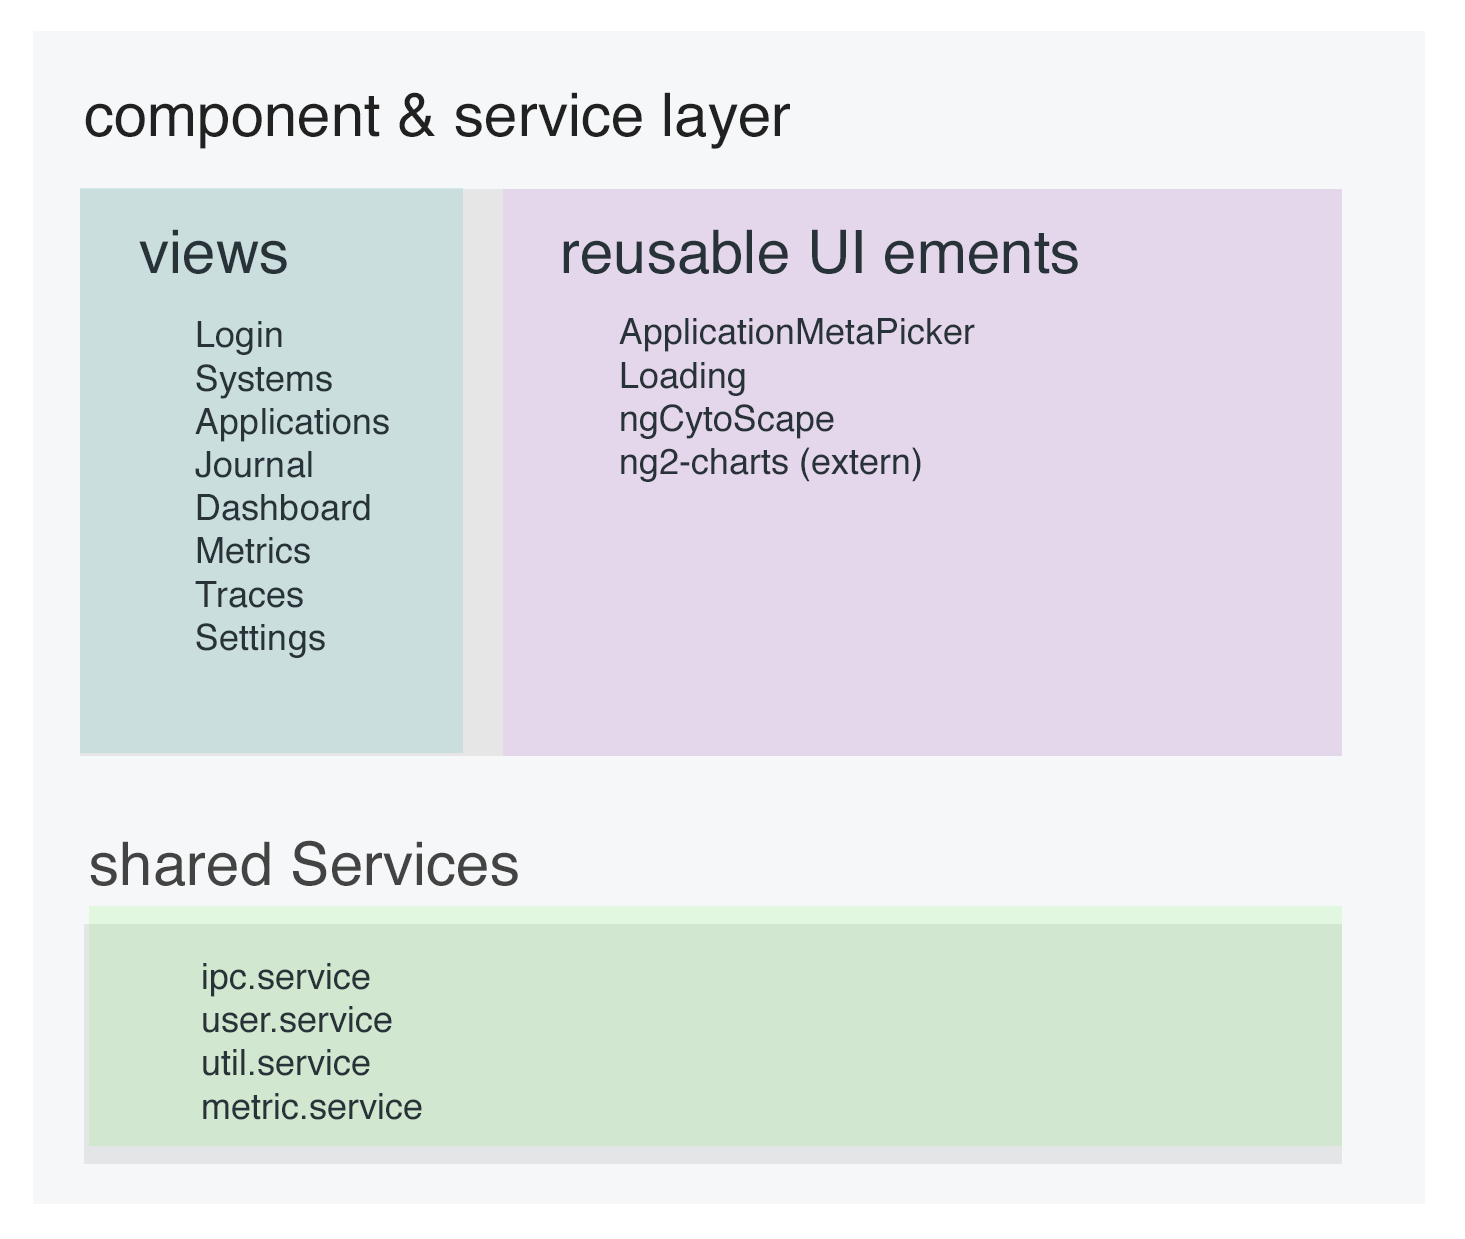
\includegraphics[width=\linewidth]{kapitel4/inner-arch.png}
 \caption{Komponenten und Services}
\end{figure}
\vspace{0.3cm}

\subsubsection{View-Komponenten}

\begin{itemize}
  \item Login
  \item Systems
  \item Applications
  \item Dashboard
  \item Journal
  \item Metrics
  \item Traces
\end{itemize}

\subsubsection{wiederverwendbare Komponenten}

Angular 2 Components, die anhand ihres Selektors in View-Komponenten eingebunden werden,
werden in \projectname{} als wiederverwendbare Komponenten bezeichnet.
Wiederverwendbar deshalb, da ihre Funktionalität lediglich anhand des Selektors eingebunden werden kann.
Wiederkehrende Elemente in den Views sollen daher in Form von wiederverwendbaren Komponenten implementiert werden.

\paragraph{ApplicationMetaPicker}




\paragraph{ngCytoScape}
\paragraph{ng2-charts}




\section{Komponenten entwickeln}


\section{Komponenten verteilen}

Um redundanten Code zu vermeiden sollen Komponenten aus der Angular 2 Applikation in der Ionic 2 App Verwendung finden.
Hierzu soll ein möglicher Workflow entwickelt und evaluiert werden, welcher Änderungen
der Angular 2 Codebase als Updates für das Ionic Projekt propagiert.

\subsection{vorbereiten}

Die zu verteilenden Komponenten sind in Typescript geschrieben,
daher müssen sie entweder im Zielprojekt in die Transpilierung mit einbezogen werden,
oder bereits vor der Verteilung transpiliert und als JavaScript Paket veröffentlicht werden.
Interessant hierbei sind die Optionen \textbf{sourceMap} und \textbf{declaration} des Typescript Transpilers.
Sind diese aktiviert, werden neben den transpilierten .js Javascript Dateien jeweils d.ts und .map Dateien abgelegt.

\paragraph{Declaration(d.ts)}

Eine d.ts Datei wird als TypeScript Declaration File bezeichnet.
Es beschreibt Implementierungen, welche in JavaScript geschrieben sind oder von TypeScript zu JavaScript transpiliert wurden.
Das Declaration File ermöglicht die Verwendung von JavaScript Code, beispielswiese einer externen Bibliothek,
in ein Projekt, welches in TypeScript geschrieben ist. Das Declaration File fungiert dabei als Interface
für die JavaScript Implementierung und gewährleistet statische Typisierung
und Autovervollständigung in unterstützenden IDEs.

Im TypeScript Transpilierungsprozess können Declaration Files mithilfe der Option \textbf{declaration} generiert werden.
Für viele populäre JavaScript Bibliotheken wurden bereits Declaration Files, von der Community oder von dem ursprünglichen Autor, nachgeliefert.
\cite[471]{EssentialTS}

\paragraph{SourceMap (.map)}

Durch die Verwendung von *-to-JavaScript Compiler/Transpiler und Minifizierungstools, ensteht ein Problem, welches SourceMaps zu lösen versuchen.
Der zur Entwicklungszeit geschriebene Code ist nicht der Selbe, welcher zur Laufzeit im Browser ausgeführt wird, da dieser transpiliert und womöglich minifiziert wurde.
Wenn nun Fehler der Applikation zur Laufzeit identifiziert werden, können diese nicht mehr auf den Ursprungscode abgebildet werden.
Der Typescript Compiler beinhaltet einen SourceMaps Generator, welcher beim Transpilevorgang .map Dateien erzeugt,
welche dabei als Referenztabelle zwischen Quell und Zielcode fungieren.
Öffnet man nun die Entwicklerkonsole in einem Browser, welcher SourceMaps unerstützt, kann man den ursprünglichen Code inspizieren.
\cite{Using97:online}


\subsection{verteilen}

Es wird eine Infrastruktur benötigt um Komponenten projektübergreifend verteilen zu können.
Möglich wäre die Konfiguration von Symlinks des lokalen Dateisystems um Komponenten in das Angular,
sowie Ionic Projekt zu integrieren. Symlinks lassen sich allerdings nicht versionieren, daher würde
für jeden Entwickler, der an dem Projekt mitwirken möchte,
ein hoher initialer Konfigurationsaufwand entstehen.
Des Weiteren sollen Komponenten womöglich nicht nur in der Ionic App,
sondern in vielen weiteren auf Angular 2 basierenden Projekten wiederverwendet werden.
Eine Komponente oder ein Paket diverser Komponenten soll veröffentlicht und aktuell
gehalten werden und soll von Entwicklern genutzt werden können.

Es liegt nahe dieses Problem mithilfe eines Paketmanagers zu lösen. Angular und Ionic verwenden für das Management
ihrer Kern-Abhängigkeiten den \ac{NPM}.
Open Source Pakete können damit kostenfrei veröffentlicht und aktualisiert werden. Closed Source Pakete können
bereits für einen Aufpreis von 7\$ pro Monat genutzt werden.


\subsection{einbinden}

\ac{NPM} Module werden mit dem Befehl \textbf{npm install modul} installiert.
Sie stehen im Projekt innerhalb der Node Modules zur Verfügung.






\paragraph{HTML und CSS Inlining}
Zudem werden \ac{HTML} und \ac{CSS} referenzen der Komponente in Inline-Strings konvertiert.
Damit werden Konflikte bezüglich relativen und absoluten Referenz-Pfaden verhindert,
da diese zentral in einer Angular Applikation konfiguriert werden.
Sind Style und Markup der Komponente als Inline-String definiert,
wird diese Konfiguration bezüglich der verteilten Komponenten hinfällig.
\cite{ludoh30:online}

\begin{figure}[h]
 \centering
 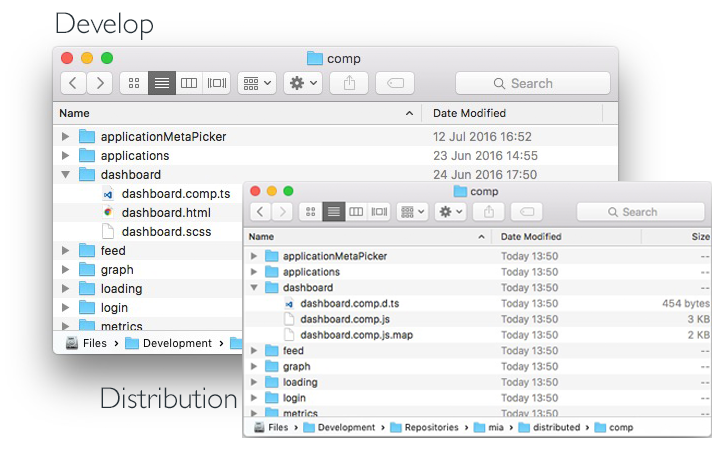
\includegraphics[width=\linewidth]{kapitel3/prepare-distribution-comp.png}
 \caption{Vergleich der Development und Distribution Komponente}
\end{figure}
\vspace{0.3cm}
